% IEEE conference template (IEEEtran). Every result number comes from tables/*.tex, which scripts/paper_tables.py
% regenerates from the saved evaluations; none is typed here. Compile: pdflatex main && bibtex main && pdflatex main (x2).
\documentclass[conference]{IEEEtran}
\usepackage[utf8]{inputenc}
\usepackage[T1]{fontenc}
\usepackage{amsmath,amssymb}
\usepackage{graphicx}
\usepackage{booktabs}
\usepackage{cite}
\usepackage{url}
\usepackage{xcolor}
\usepackage{tikz}
\usetikzlibrary{arrows.meta,positioning}

% numbers quoted in the prose, read from the same records as the tables (scripts/paper_tables.py); do not edit
\newcommand{\NApBfive}{61.93}
\newcommand{\NApBfour}{62.91}
\newcommand{\NApBthree}{65.74}
\newcommand{\NApBthreem}{64.89}
\newcommand{\NApBthreemY}{64.79}
\newcommand{\NApBzero}{0.08}
\newcommand{\NApFull}{61.94}
\newcommand{\NApFullPtwo}{61.86}
\newcommand{\NApFullY}{61.87}
\newcommand{\NApbBfive}{36.22}
\newcommand{\NApbBfour}{38.39}
\newcommand{\NApbBthree}{43.64}
\newcommand{\NApbBthreem}{41.35}
\newcommand{\NApbBthreemY}{41.05}
\newcommand{\NApbBzero}{0.05}
\newcommand{\NApbFull}{36.22}
\newcommand{\NApbFullPtwo}{36.16}
\newcommand{\NApbFullY}{36.18}
\newcommand{\NBinaryToFullAp}{-2.95}
\newcommand{\NBinaryToFullApCi}{[-3.15, -2.65]}
\newcommand{\NBinaryToFullCiou}{-2.42}
\newcommand{\NBinaryToFullCiouCi}{[-2.67, -2.16]}
\newcommand{\NBinaryToFullMerge}{-0.85}
\newcommand{\NBinaryToFullMergeCi}{[-1.01, -0.67]}
\newcommand{\NBinaryToFullMta}{+0.39}
\newcommand{\NBinaryToFullMtaCi}{[+0.26, +0.51]}
\newcommand{\NBinaryToFullPolis}{+0.138}
\newcommand{\NBinaryToFullPolisCi}{[+0.130, +0.147]}
\newcommand{\NBinaryToFullSplit}{+1.52}
\newcommand{\NBinaryToFullSplitCi}{[+1.37, +1.66]}
\newcommand{\NBinaryToFullTouchingAp}{-1.15}
\newcommand{\NBinaryToFullTouchingApCi}{[-2.21, +0.13]}
\newcommand{\NBinaryToFullTouchingCiou}{-2.32}
\newcommand{\NBinaryToFullTouchingCiouCi}{[-3.08, -1.57]}
\newcommand{\NBinaryToFullTouchingMerge}{-4.04}
\newcommand{\NBinaryToFullTouchingMergeCi}{[-5.24, -2.83]}
\newcommand{\NBinaryToFullTouchingMta}{+0.33}
\newcommand{\NBinaryToFullTouchingMtaCi}{[-0.12, +0.82]}
\newcommand{\NBinaryToFullTouchingPolis}{+0.103}
\newcommand{\NBinaryToFullTouchingPolisCi}{[+0.073, +0.131]}
\newcommand{\NBinaryToFullTouchingSplit}{+1.35}
\newcommand{\NBinaryToFullTouchingSplitCi}{[+0.83, +1.96]}
\newcommand{\NCiouBfive}{73.87}
\newcommand{\NCiouBfour}{62.69}
\newcommand{\NCiouBthree}{66.51}
\newcommand{\NCiouBthreem}{76.97}
\newcommand{\NCiouBthreemY}{76.88}
\newcommand{\NCiouBzero}{6.93}
\newcommand{\NCiouFull}{74.55}
\newcommand{\NCiouFullPtwo}{74.22}
\newcommand{\NCiouFullY}{74.48}
\newcommand{\NCleanApFull}{61.14}
\newcommand{\NCleanApHisup}{65.60}
\newcommand{\NCleanApbFull}{35.19}
\newcommand{\NCleanApbHisup}{43.97}
\newcommand{\NCleanApfiftyFull}{86.15}
\newcommand{\NCleanApfiftyHisup}{87.29}
\newcommand{\NCleanCiouFull}{73.29}
\newcommand{\NCleanCiouHisup}{81.25}
\newcommand{\NCleanDeltaAp}{-4.45}
\newcommand{\NCleanDeltaApCi}{[-5.73, -3.44]}
\newcommand{\NCleanDeltaApb}{-8.79}
\newcommand{\NCleanDeltaApbCi}{[-10.55, -7.41]}
\newcommand{\NCleanDeltaPolis}{+0.461}
\newcommand{\NCleanDeltaPolisCi}{[+0.325, +0.587]}
\newcommand{\NContactInactive}{6}
\newcommand{\NContactRuns}{9}
\newcommand{\NDenseMerge}{+0.03}
\newcommand{\NDenseMergeCi}{[-0.27, +0.31]}
\newcommand{\NDenseMergeDense}{+0.15}
\newcommand{\NDenseMergeMedium}{+0.10}
\newcommand{\NDenseMergeSparse}{+0.12}
\newcommand{\NDenseMta}{-0.51}
\newcommand{\NDenseMtaCi}{[-0.85, -0.19]}
\newcommand{\NDenseMtaDense}{-0.94}
\newcommand{\NDenseMtaMedium}{-0.73}
\newcommand{\NDenseMtaSparse}{-0.42}
\newcommand{\NDensePolis}{-0.025}
\newcommand{\NDensePolisCi}{[-0.054, +0.006]}
\newcommand{\NDensePolisDense}{-0.037}
\newcommand{\NDensePolisMedium}{-0.021}
\newcommand{\NDensePolisSparse}{-0.012}
\newcommand{\NDetectorMap}{0.917}
\newcommand{\NDetectorRecall}{0.849}
\newcommand{\NFpsBthree}{74.0}
\newcommand{\NFpsFull}{42.3}
\newcommand{\NFpsFullY}{36.4}
\newcommand{\NIouBfive}{88.04}
\newcommand{\NIouBfour}{88.46}
\newcommand{\NIouBthree}{89.89}
\newcommand{\NIouBthreem}{89.43}
\newcommand{\NIouBthreemY}{89.43}
\newcommand{\NIouBzero}{22.49}
\newcommand{\NIouFull}{88.01}
\newcommand{\NIouFullPtwo}{87.99}
\newcommand{\NIouFullY}{88.01}
\newcommand{\NLeakyApHisup}{79.43}
\newcommand{\NMergeBfive}{2.05}
\newcommand{\NMergeBfour}{2.07}
\newcommand{\NMergeBthree}{2.84}
\newcommand{\NMergeBthreem}{2.81}
\newcommand{\NMergeBthreemY}{2.14}
\newcommand{\NMergeBzero}{0.02}
\newcommand{\NMergeFull}{1.96}
\newcommand{\NMergeFullPtwo}{2.09}
\newcommand{\NMergeFullY}{1.52}
\newcommand{\NMergeTouchingBfive}{8.07}
\newcommand{\NMergeTouchingBfour}{8.23}
\newcommand{\NMergeTouchingBthree}{12.13}
\newcommand{\NMergeTouchingBthreem}{11.86}
\newcommand{\NMergeTouchingBthreemY}{8.92}
\newcommand{\NMergeTouchingBzero}{0.22}
\newcommand{\NMergeTouchingFull}{7.81}
\newcommand{\NMergeTouchingFullPtwo}{8.32}
\newcommand{\NMergeTouchingFullY}{6.41}
\newcommand{\NMtaBfive}{37.30}
\newcommand{\NMtaBfour}{47.11}
\newcommand{\NMtaBthree}{45.51}
\newcommand{\NMtaBthreem}{36.16}
\newcommand{\NMtaBthreemY}{36.14}
\newcommand{\NMtaBzero}{41.12}
\newcommand{\NMtaFull}{36.34}
\newcommand{\NMtaFullPtwo}{36.22}
\newcommand{\NMtaFullY}{36.31}
\newcommand{\NNoneGuideAp}{-0.04}
\newcommand{\NNoneGuideApCi}{[-0.13, +0.07]}
\newcommand{\NNoneGuideMta}{-0.18}
\newcommand{\NNoneGuideMtaCi}{[-0.27, -0.09]}
\newcommand{\NNoneGuidePolis}{-0.017}
\newcommand{\NNoneGuidePolisCi}{[-0.019, -0.015]}
\newcommand{\NNoneTotalAp}{+0.35}
\newcommand{\NNoneTotalApCi}{[+0.11, +0.54]}
\newcommand{\NNoneTotalMta}{-0.94}
\newcommand{\NNoneTotalMtaCi}{[-1.10, -0.78]}
\newcommand{\NNoneTotalPolis}{-0.037}
\newcommand{\NNoneTotalPolisCi}{[-0.044, -0.030]}
\newcommand{\NNoneTrainAp}{+0.40}
\newcommand{\NNoneTrainApCi}{[+0.13, +0.56]}
\newcommand{\NNoneTrainMta}{-0.77}
\newcommand{\NNoneTrainMtaCi}{[-0.92, -0.63]}
\newcommand{\NNoneTrainPolis}{-0.020}
\newcommand{\NNoneTrainPolisCi}{[-0.027, -0.013]}
\newcommand{\NNratioBfive}{1.27}
\newcommand{\NNratioBfour}{1.83}
\newcommand{\NNratioBthree}{1.70}
\newcommand{\NNratioBthreem}{1.19}
\newcommand{\NNratioBthreemY}{1.20}
\newcommand{\NNratioBzero}{9.82}
\newcommand{\NNratioFull}{1.26}
\newcommand{\NNratioFullPtwo}{1.27}
\newcommand{\NNratioFullY}{1.26}
\newcommand{\NNthreeDeltaAp}{-0.08}
\newcommand{\NNthreeDeltaApCi}{[-0.27, +0.08]}
\newcommand{\NNthreeDeltaMerge}{+0.15}
\newcommand{\NNthreeDeltaMergeCi}{[+0.02, +0.30]}
\newcommand{\NParamsBthree}{20.81}
\newcommand{\NParamsFull}{20.81}
\newcommand{\NParamsFullY}{20.81}
\newcommand{\NPolisBfive}{1.836}
\newcommand{\NPolisBfour}{1.903}
\newcommand{\NPolisBthree}{1.697}
\newcommand{\NPolisBthreem}{1.657}
\newcommand{\NPolisBthreemY}{1.678}
\newcommand{\NPolisBzero}{3.525}
\newcommand{\NPolisFull}{1.823}
\newcommand{\NPolisFullPtwo}{1.815}
\newcommand{\NPolisFullY}{1.850}
\newcommand{\NRegBinaryAp}{-0.85}
\newcommand{\NRegBinaryApCi}{[-1.01, -0.70]}
\newcommand{\NRegBinaryCiou}{+10.46}
\newcommand{\NRegBinaryCiouCi}{[+10.09, +10.81]}
\newcommand{\NRegBinaryMerge}{-0.03}
\newcommand{\NRegBinaryMergeCi}{[-0.06, -0.00]}
\newcommand{\NRegBinaryMta}{-9.39}
\newcommand{\NRegBinaryMtaCi}{[-9.55, -9.23]}
\newcommand{\NRegBinaryPolis}{-0.042}
\newcommand{\NRegBinaryPolisCi}{[-0.046, -0.038]}
\newcommand{\NRegBinarySplit}{+0.01}
\newcommand{\NRegBinarySplitCi}{[-0.01, +0.02]}
\newcommand{\NRegBinaryTouchingAp}{-0.69}
\newcommand{\NRegBinaryTouchingApCi}{[-0.97, -0.51]}
\newcommand{\NRegBinaryTouchingCiou}{+10.23}
\newcommand{\NRegBinaryTouchingCiouCi}{[+8.81, +11.67]}
\newcommand{\NRegBinaryTouchingMerge}{-0.27}
\newcommand{\NRegBinaryTouchingMergeCi}{[-0.49, -0.09]}
\newcommand{\NRegBinaryTouchingMta}{-9.60}
\newcommand{\NRegBinaryTouchingMtaCi}{[-10.22, -9.04]}
\newcommand{\NRegBinaryTouchingPolis}{-0.059}
\newcommand{\NRegBinaryTouchingPolisCi}{[-0.072, -0.047]}
\newcommand{\NRegBinaryTouchingSplit}{-0.04}
\newcommand{\NRegBinaryTouchingSplitCi}{[-0.13, +0.05]}
\newcommand{\NSeedBinaryAp}{-0.10}
\newcommand{\NSeedBinaryApCi}{[-0.28, +0.20]}
\newcommand{\NSeedBinaryCiou}{-0.08}
\newcommand{\NSeedBinaryCiouCi}{[-0.13, -0.04]}
\newcommand{\NSeedBinaryMerge}{-0.67}
\newcommand{\NSeedBinaryMergeCi}{[-0.82, -0.53]}
\newcommand{\NSeedBinaryMta}{-0.01}
\newcommand{\NSeedBinaryMtaCi}{[-0.01, -0.00]}
\newcommand{\NSeedBinaryPolis}{+0.003}
\newcommand{\NSeedBinaryPolisCi}{[-0.002, +0.008]}
\newcommand{\NSeedBinarySplit}{+0.36}
\newcommand{\NSeedBinarySplitCi}{[+0.30, +0.44]}
\newcommand{\NSeedBinaryTouchingAp}{+1.64}
\newcommand{\NSeedBinaryTouchingApCi}{[+0.52, +3.26]}
\newcommand{\NSeedBinaryTouchingCiou}{+0.07}
\newcommand{\NSeedBinaryTouchingCiouCi}{[-0.18, +0.36]}
\newcommand{\NSeedBinaryTouchingMerge}{-2.94}
\newcommand{\NSeedBinaryTouchingMergeCi}{[-4.49, -1.64]}
\newcommand{\NSeedBinaryTouchingMta}{-0.01}
\newcommand{\NSeedBinaryTouchingMtaCi}{[-0.04, +0.01]}
\newcommand{\NSeedBinaryTouchingPolis}{-0.024}
\newcommand{\NSeedBinaryTouchingPolisCi}{[-0.042, -0.006]}
\newcommand{\NSeedBinaryTouchingSplit}{+0.49}
\newcommand{\NSeedBinaryTouchingSplitCi}{[+0.13, +0.96]}
\newcommand{\NSeedFullAp}{-0.07}
\newcommand{\NSeedFullApCi}{[-0.24, +0.05]}
\newcommand{\NSeedFullCiou}{-0.07}
\newcommand{\NSeedFullCiouCi}{[-0.12, -0.04]}
\newcommand{\NSeedFullMerge}{-0.45}
\newcommand{\NSeedFullMergeCi}{[-0.56, -0.35]}
\newcommand{\NSeedFullMta}{-0.01}
\newcommand{\NSeedFullMtaCi}{[-0.02, -0.00]}
\newcommand{\NSeedFullPolis}{+0.008}
\newcommand{\NSeedFullPolisCi}{[+0.003, +0.014]}
\newcommand{\NSeedFullSplit}{+0.24}
\newcommand{\NSeedFullSplitCi}{[+0.19, +0.30]}
\newcommand{\NSeedFullTouchingAp}{+0.66}
\newcommand{\NSeedFullTouchingApCi}{[-0.06, +1.34]}
\newcommand{\NSeedFullTouchingCiou}{-0.09}
\newcommand{\NSeedFullTouchingCiouCi}{[-0.28, +0.05]}
\newcommand{\NSeedFullTouchingMerge}{-1.41}
\newcommand{\NSeedFullTouchingMergeCi}{[-2.21, -0.72]}
\newcommand{\NSeedFullTouchingMta}{-0.02}
\newcommand{\NSeedFullTouchingMtaCi}{[-0.05, +0.00]}
\newcommand{\NSeedFullTouchingPolis}{-0.007}
\newcommand{\NSeedFullTouchingPolisCi}{[-0.033, +0.026]}
\newcommand{\NSeedFullTouchingSplit}{+0.18}
\newcommand{\NSeedFullTouchingSplitCi}{[+0.02, +0.42]}
\newcommand{\NSeededPairAp}{-2.92}
\newcommand{\NSeededPairApCi}{[-3.17, -2.72]}
\newcommand{\NSeededPairCiou}{-2.41}
\newcommand{\NSeededPairCiouCi}{[-2.65, -2.15]}
\newcommand{\NSeededPairMerge}{-0.63}
\newcommand{\NSeededPairMergeCi}{[-0.76, -0.49]}
\newcommand{\NSeededPairMta}{+0.38}
\newcommand{\NSeededPairMtaCi}{[+0.26, +0.50]}
\newcommand{\NSeededPairPolis}{+0.144}
\newcommand{\NSeededPairPolisCi}{[+0.136, +0.154]}
\newcommand{\NSeededPairSplit}{+1.39}
\newcommand{\NSeededPairSplitCi}{[+1.25, +1.54]}
\newcommand{\NSeededPairTouchingAp}{-2.13}
\newcommand{\NSeededPairTouchingApCi}{[-2.92, -1.49]}
\newcommand{\NSeededPairTouchingCiou}{-2.48}
\newcommand{\NSeededPairTouchingCiouCi}{[-3.30, -1.68]}
\newcommand{\NSeededPairTouchingMerge}{-2.51}
\newcommand{\NSeededPairTouchingMergeCi}{[-3.34, -1.68]}
\newcommand{\NSeededPairTouchingMta}{+0.33}
\newcommand{\NSeededPairTouchingMtaCi}{[-0.13, +0.80]}
\newcommand{\NSeededPairTouchingPolis}{+0.123}
\newcommand{\NSeededPairTouchingPolisCi}{[+0.089, +0.160]}
\newcommand{\NSeededPairTouchingSplit}{+1.05}
\newcommand{\NSeededPairTouchingSplitCi}{[+0.51, +1.66]}
\newcommand{\NSelectTiles}{1,928}
\newcommand{\NTestTiles}{2,928}
\newcommand{\NTilesClean}{212}
\newcommand{\NTilesDense}{857}
\newcommand{\NTilesTouching}{146}
\newcommand{\NTrainClusters}{29,283}
\newcommand{\NTrainDedup}{23,427}
\newcommand{\NTrainImages}{280,741}
\newcommand{\NTuneTiles}{1,000}
\newcommand{\NValImages}{60,317}
\newcommand{\NWhuAp}{66.97}
\newcommand{\NWhuCiou}{66.83}
\newcommand{\NWhuCiouHisup}{79.62}
\newcommand{\NWhuCiouMain}{72.07}
\newcommand{\NWhuCiouPixtopoly}{81.63}
\newcommand{\NWhuIou}{83.92}
\newcommand{\NWhuMerge}{3.04}
\newcommand{\NWhuMergeTouching}{14.73}
\newcommand{\NWhuPatches}{29,088}


% Working title of the paper; the registered title of the course project is in Indonesian (see README).
\newcommand{\papertitle}{Building Polygon Extraction in Dense Settlements Without Polygon Annotations:
A Leakage-Free, Density-Stratified Evaluation of Orientation-Guided Regularization}

\begin{document}

\title{\papertitle}

\author{\IEEEauthorblockN{Mahathir Muhammad}
\IEEEauthorblockA{Department of Informatics\\
Institut Teknologi Sepuluh Nopember\\
Surabaya, Indonesia}}

\maketitle

\begin{abstract}
Polygonal building extraction is usually trained with polygon annotations and reported on the CrowdAI benchmark, whose
validation set overlaps its training set. We study what can be had from instance masks alone, and how much of the
reported accuracy survives a leakage-free protocol. Our pipeline segments buildings with a U-Net++, separates them with
a contact class and a watershed, predicts a per-pixel orientation whose labels are derived from the masks, and uses it
to regularize each contour into a polygon. On a deduplicated CrowdAI split with decision rules fixed before any result,
three seeds and paired bootstrap intervals, the orientation head lowers the paired PoLiS by $\NNoneTotalPolis$\,px and
the per-instance tangent angle error by $\NNoneTotalMta^\circ$ in dense tiles; the effect is small but consistent, and
it grows with building density. Two other ideas do not hold: morphological priors added to the input do not reduce
merged buildings, and the contact class stays inactive in most runs. An exploratory baseline, a binary segmentation
whose components are regularized with minimum-area rectangles, beats the full pipeline on every metric but merged
buildings (AP \NApBthreem{} against \NApFull). Seeds from an oriented-box detector, also trained from masks, cut merged
buildings by about a quarter at equal AP. On \NTilesClean{} validation tiles without a duplicate in training, HiSup
scores \NCleanApHisup{} AP instead of the \NLeakyApHisup{} of the full validation set, and our mask-supervised
pipeline is $\NCleanDeltaAp$ AP behind it.
\end{abstract}

\begin{IEEEkeywords}
building extraction, polygon regularization, instance segmentation, data leakage, remote sensing
\end{IEEEkeywords}

\section{Introduction}
Maps need buildings as polygons with few vertices and straight walls, not as masks. Recent methods learn polygons
directly~\cite{girard2021ffl,zorzi2022polyworld,xu2023hisup,jiao2024polyrcnn,adimoolam2025pix2poly} and report an average
precision close to 80 on the CrowdAI Mapping Challenge~\cite{mohanty2020crowdai}. Two facts qualify these numbers. First,
they need polygon annotations, which many regional datasets lack. Second, the CrowdAI validation set shares most of its
images with the training set, up to rotations and flips~\cite{adimoolam2023leakage}, so the benchmark rewards
memorization.

This paper asks two questions about dense settlements, where roofs touch and a single merged polygon hides several
houses. How good can polygons be when only instance masks are available for training? And which design choices of a
mask-supervised pipeline survive an evaluation without leakage, split by building density?

We built a pipeline from known parts and three additions of our own, wrote down beforehand how each addition would be
judged, and then ran the experiments. The outcome is mixed, and we report it as such:
\begin{itemize}
\item \textbf{Protocol.} A CrowdAI split without duplicate tiles across training, tuning and test, density strata frozen
from the ground truth, three seeds, paired cluster-bootstrap intervals, and decision rules fixed before any model was
trained (Section~\ref{sec:protocol}).
\item \textbf{Orientation from masks.} A two-channel head predicts the building orientation, with labels derived from the
minimum-area rectangle of each mask, and guides the regularization. It improves polygon geometry by a small, consistent
amount that grows with density (Section~\ref{sec:n1}).
\item \textbf{Negative results.} Morphological priors as extra input channels do not help, and the contact class meant to
separate touching roofs is rarely predicted at all (Sections~\ref{sec:n3} and~\ref{sec:contact}).
\item \textbf{A simple strong baseline.} Regularizing the connected components of a binary segmentation is better than
the full pipeline on every metric except merged buildings, and detector seeds reduce merges in both
(Section~\ref{sec:exploratory}). These comparisons were added after the results and are marked as exploratory.
\end{itemize}

\section{Related Work}
\textbf{Polygonal building extraction.} Frame field learning~\cite{girard2021ffl} predicts a field aligned with building
walls and polygonizes the mask with it. PolyWorld~\cite{zorzi2022polyworld}, HiSup~\cite{xu2023hisup},
PolyR-CNN~\cite{jiao2024polyrcnn} and Pix2Poly~\cite{adimoolam2025pix2poly} predict vertices and their connections more
directly. All of them are trained with polygon annotations. Our orientation head is a much reduced relative of the frame
field: one angle modulo $90^\circ$ per pixel, supervised by rectangles fitted to masks.

\textbf{Separating touching buildings.} A third class for the pixels where instances meet, followed by a watershed, was
introduced for satellite imagery by TernausNetV2~\cite{iglovikov2018ternausv2}; weighting the loss near
boundaries goes back to U-Net~\cite{ronneberger2015unet} and was applied to footprints by Bischke et
al.~\cite{bischke2019multitask}. We adopt both without claiming them.

\textbf{Morphological cues.} The morphological building index (MBI)~\cite{huang2011mbi} responds to bright structures of
building size. We test it, and a directional black top-hat that responds to the dark gaps between roofs, as extra input
channels.

\textbf{Leakage in CrowdAI.} Adimoolam et al.~\cite{adimoolam2023leakage} showed with perceptual hashes that most
CrowdAI training images are exact or augmented duplicates and that the validation set leaks from the training set. We
build on their finding and re-evaluate a published method on the validation tiles that are free of it.

\section{Method}
\label{sec:method}
Fig.~\ref{fig:pipeline} shows the pipeline. Everything it learns from is derived from an instance map, one integer label
per building; no polygon annotation is used in training.

\begin{figure}[t]
\centering
\resizebox{\columnwidth}{!}{%
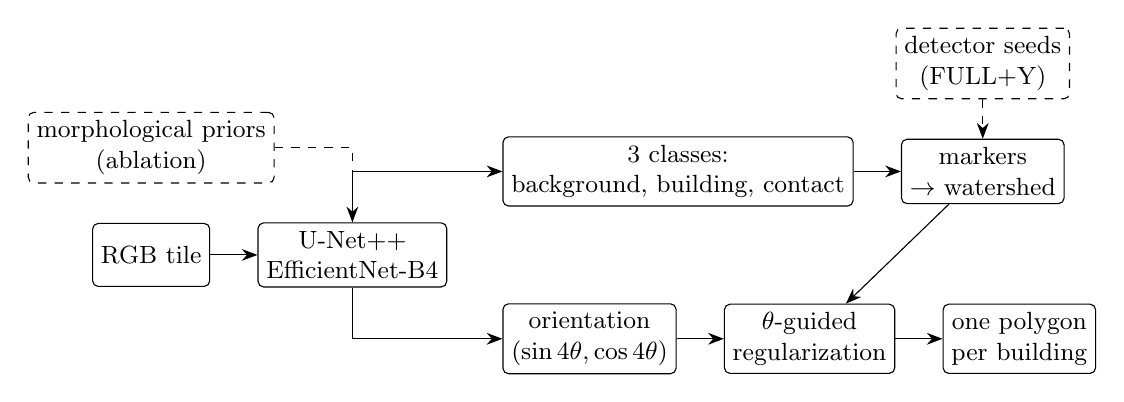
\begin{tikzpicture}[node distance=5mm and 6mm, >={Stealth[length=2mm]},
  box/.style={draw, rounded corners=2pt, align=center, font=\small, minimum height=8mm, inner sep=3pt},
  opt/.style={box, dashed}]
\node[box] (rgb) {RGB tile};
\node[box, right=of rgb] (net) {U-Net++\\EfficientNet-B4};
\node[box, above right=2mm and 7mm of net] (cls) {3 classes:\\background, building, contact};
\node[box, below right=2mm and 7mm of net] (ori) {orientation\\$(\sin 4\theta,\cos 4\theta)$};
\node[box, right=of cls] (ws) {markers\\$\rightarrow$ watershed};
\node[box, right=of ori] (reg) {$\theta$-guided\\regularization};
\node[box, right=of reg] (out) {one polygon\\per building};
\node[opt, above=of ws] (det) {detector seeds\\(FULL+Y)};
\node[opt, above=of rgb] (pri) {morphological priors\\(ablation)};
\draw[->] (rgb) -- (net);
\draw[->] (net) |- (cls);
\draw[->] (net) |- (ori);
\draw[->] (cls) -- (ws);
\draw[->] (ws) -- (reg);
\draw[->] (ori) -- (reg);
\draw[->] (reg) -- (out);
\draw[->, dashed] (det) -- (ws);
\draw[->, dashed] (pri) -| (net);
\end{tikzpicture}}
\caption{The mask-supervised pipeline. Dashed parts are variants: morphological priors as extra input channels, and
seeds from an oriented-box detector. All labels, including the orientation and the detector's boxes, come from instance
masks.}
\label{fig:pipeline}
\end{figure}

\subsection{Labels from masks}
\textbf{Classes.} A pixel is background, building or contact. Contact pixels are building pixels within $r$ pixels of
another building ($r=2$ on CrowdAI).

\textbf{Orientation.} For each instance we fit the minimum-area rectangle and take the direction $\theta$ of one of its
sides, modulo $90^\circ$. The targets are $(\sin 4\theta,\cos 4\theta)$ on the pixels of the instance, which removes
the ambiguity between the four sides. Labels are derived after the geometric augmentation, so that flips and
transpositions are handled without special cases.

\textbf{Boundary weight.} Each pixel has a weight $w=1+\alpha\exp(-d^2/2\sigma^2)$, where $d$ is the distance to the
nearest instance boundary ($\alpha=5$, $\sigma=3$\,px).

\subsection{Network and loss}
The network is a U-Net++~\cite{zhou2018unetpp} with an EfficientNet-B4 encoder~\cite{tan2019efficientnet} pretrained on
ImageNet, and one convolutional head with five outputs: three class logits and two orientation channels through a
$\tanh$. The loss is
\begin{equation}
L = \overline{w\cdot\mathrm{CE}} + L_{\mathrm{Dice}} + \lambda L_\theta ,
\end{equation}
where $L_\theta$ is the mean squared error of the two orientation channels over building pixels and $\lambda=1$.

\subsection{Instances}
With class probabilities $P_{bg}$, $P_b$, $P_k$, the foreground is $1-P_{bg}>0.5$ and the markers are the components of
$P_b-P_k>\tau$ inside it. A watershed of $-P_b$ from the markers, restricted to the foreground, gives the instances;
foreground components without a marker become instances of their own.

\subsection{Orientation-guided regularization}
The orientation of an instance is the circular mean of the head's output over its pixels. In the frame rotated by
$-\theta$, the contour is first compared with a rectangle whose sides come from the second-order moments of the mask; if
their IoU reaches $\rho$, the rectangle is the polygon. Otherwise the contour is simplified with
Douglas--Peucker~\cite{douglas1973}, with a tolerance proportional to the square root of the area, its edges within
$\delta$ of the two axes are snapped to them, consecutive edges of the same class are merged, and the vertices are
recomputed as intersections. A result that is invalid or leaves the contour (IoU below 0.7) falls back to the simplified
contour. The same procedure with $\theta$ taken from the minimum-area rectangle of the predicted instance, instead of
the head, is the mode we call \emph{mar}.

\subsection{Variants}
\textbf{Morphological priors.} MBI and a gap map, the difference between the largest and the smallest directional black
top-hat, are appended to the RGB input. The first convolution is widened with zero weights for the new channels, so
that the pretrained network is unchanged at the start of training.

\textbf{Detector seeds.} A YOLOv8n oriented-box detector~\cite{jocher2023yolov8} is trained on boxes fitted to the same
instance masks. At inference the centres of its boxes become seeds: a marker that contains two or more seeds is replaced
by them, and a seed in a foreground component without a marker is added.

\section{Evaluation Protocol}
\label{sec:protocol}
\subsection{Data without leakage}
CrowdAI~\cite{mohanty2020crowdai} has \NTrainImages{} training and \NValImages{} validation tiles of $300\times300$
pixels. We hash every training tile and its eight rotations and flips with a perceptual hash, as
in~\cite{adimoolam2023leakage}, and obtain \NTrainClusters{} clusters of duplicates. One tile per cluster is kept. The
clusters are shuffled once: 10\% form the tuning split, divided into \NTuneTiles{} tiles for tuning the post-processing
and \NSelectTiles{} for selecting checkpoints, another 10\% (\NTestTiles{} tiles) form the test split, and the remaining
\NTrainDedup{} tiles are used for training. No parameter is tuned on the test split.

The published methods were trained on the full training set, so our test split is not clean for them. For the
comparison with HiSup~\cite{xu2023hisup}, whose predictions on the validation set are public, we use the validation
tiles that have no duplicate in the training set even after rotations and flips, one per cluster: \NTilesClean{} tiles.

The WHU aerial dataset~\cite{ji2019whu} serves as a second dataset with one seed. Following
Pix2Poly~\cite{adimoolam2025pix2poly} we evaluate on $224\times224$ patches, but our test tiles are rebuilt from the
official release and are not exactly theirs, so the comparison with their reported numbers is approximate.

\subsection{Density strata}
Before any model was evaluated, the test tiles were divided into terciles by their number of ground-truth buildings
(sparse, medium, dense), and, as a second index, into tiles with and without touching buildings.

\subsection{Metrics}
We report the COCO mask AP~\cite{lin2014coco} and its boundary variant~\cite{cheng2021boundaryiou}, the pixel IoU, the
complexity-aware IoU and the vertex ratio of~\cite{zorzi2022polyworld}, PoLiS~\cite{avbelj2015polis} and the max tangent
angle error (MTA)~\cite{girard2021ffl}, computed with the scripts of Pix2Poly. Since those pooled versions of PoLiS and
MTA depend on which buildings a method finds, the claims use paired versions: predictions are matched one-to-one to the
ground truth at an IoU of 0.5, and PoLiS and MTA are averaged over the buildings matched by both methods compared. The
merge rate is the share of ground-truth buildings covered by a prediction that also covers another building, and the
split rate the share covered by two or more predictions.

\subsection{Statistics and decision rules}
Core comparisons use three seeds. Differences are paired by seed and averaged; their 95\% interval comes from a cluster
bootstrap over tiles with 1000 replicates, the same resamples for both methods. The rules were written down before any
model was trained: a contribution is supported if, in the dense stratum of the test split, its main metrics improve
with an interval that excludes zero and in all three seeds, and AP does not fall by more than 0.5 points. ``Largest in
dense areas'' needs the interval of the difference between the dense and the sparse effect to exclude zero for every
main metric. ``Close to the state of the art'' means at most 3 AP behind HiSup on the clean validation tiles.
Comparisons outside this list are exploratory and marked as such.

\subsection{Training}
All CrowdAI models are trained for 60 epochs with AdamW~\cite{loshchilov2019adamw}, a batch of 16, a learning rate of
$2\times10^{-4}$ with one warm-up epoch and a cosine decay, mixed precision, and flips, right-angle rotations,
transpositions and a mild photometric jitter. Tiles are padded to $320\times320$, never resized. The checkpoint with the
best foreground IoU on the selection split is kept. The post-processing of every model is tuned on the same grid.
Table~\ref{tab:ablation} lists the scenarios: B0 is a classical MBI baseline, B1--B3 are binary segmentations (U-Net,
U-Net++, with boundary weights), B4 adds the contact class and the watershed, B5 regularizes B4 in mode \emph{mar}, and
FULL adds the orientation head, without priors (P0), with MBI (P1), or with MBI and the gap map (P2).
B5$'$ applies mode \emph{mar} to the FULL-P0 network, which separates the effect of training with the head from the
effect of using its output.

\section{Results}
\begin{table*}[t]
\centering
\caption{Scenarios on the deduplicated CrowdAI test split (mean $\pm$ standard deviation over the runs). AP, IoU, C-IoU
and merge rate in percent, PoLiS in pixels, MTA in degrees. FULL+Y adds detector seeds; B3m and B3m+Y are exploratory.}
\label{tab:ablation}
\resizebox{\textwidth}{!}{% ablation: from tables/crowdai/ablation.json (git f96e54a20f99, 2026-11-12T20:27:37+07:00); do not edit
\begin{tabular}{l c ccccccccc}
\toprule
Code & Runs & AP & AP$_{50}$ & AP$_b$ & IoU & PoLiS$\downarrow$ & MTA$\downarrow$ & C-IoU & N-ratio & Merge$\downarrow$ \\
\midrule
B0 & 1 & 0.08 & 0.26 & 0.05 & 22.49 & 3.525 & 41.12 & 6.93 & 9.82 & 0.02 \\
\midrule
B1 & 1 & 63.54 & 85.44 & 39.68 & 89.38 & 1.790 & 46.02 & 67.81 & 1.60 & 3.05 \\
B2 & 1 & 63.23 & 85.36 & 38.95 & 89.22 & 1.799 & 46.45 & 67.00 & 1.64 & 3.28 \\
B3 & 3 & 65.74\,{\scriptsize$\pm$0.07} & 87.21\,{\scriptsize$\pm$0.05} & 43.64\,{\scriptsize$\pm$0.22} & 89.89\,{\scriptsize$\pm$0.06} & 1.697\,{\scriptsize$\pm$0.008} & 45.51\,{\scriptsize$\pm$0.25} & 66.51\,{\scriptsize$\pm$0.33} & 1.70\,{\scriptsize$\pm$0.02} & 2.84\,{\scriptsize$\pm$0.15} \\
\midrule
B4 & 3 & 62.91\,{\scriptsize$\pm$0.32} & 86.16\,{\scriptsize$\pm$0.06} & 38.39\,{\scriptsize$\pm$0.61} & 88.46\,{\scriptsize$\pm$0.18} & 1.903\,{\scriptsize$\pm$0.028} & 47.11\,{\scriptsize$\pm$0.13} & 62.69\,{\scriptsize$\pm$0.26} & 1.83\,{\scriptsize$\pm$0.01} & 2.07\,{\scriptsize$\pm$0.03} \\
B5 & 3 & 61.93\,{\scriptsize$\pm$0.31} & 86.12\,{\scriptsize$\pm$0.06} & 36.22\,{\scriptsize$\pm$0.49} & 88.04\,{\scriptsize$\pm$0.17} & 1.836\,{\scriptsize$\pm$0.018} & 37.30\,{\scriptsize$\pm$0.13} & 73.87\,{\scriptsize$\pm$0.10} & 1.27\,{\scriptsize$\pm$0.01} & 2.05\,{\scriptsize$\pm$0.06} \\
B5$'$ & 3 & 62.04\,{\scriptsize$\pm$0.67} & 86.12\,{\scriptsize$\pm$0.02} & 36.21\,{\scriptsize$\pm$1.21} & 88.03\,{\scriptsize$\pm$0.36} & 1.844\,{\scriptsize$\pm$0.042} & 36.63\,{\scriptsize$\pm$0.22} & 74.40\,{\scriptsize$\pm$0.67} & 1.25\,{\scriptsize$\pm$0.02} & 1.94\,{\scriptsize$\pm$0.21} \\
\midrule
FULL-P0 & 3 & 61.94\,{\scriptsize$\pm$0.68} & 86.12\,{\scriptsize$\pm$0.02} & 36.22\,{\scriptsize$\pm$1.19} & 88.01\,{\scriptsize$\pm$0.35} & 1.823\,{\scriptsize$\pm$0.044} & 36.34\,{\scriptsize$\pm$0.24} & 74.55\,{\scriptsize$\pm$0.64} & 1.26\,{\scriptsize$\pm$0.03} & 1.96\,{\scriptsize$\pm$0.20} \\
FULL-P1 & 3 & 62.10\,{\scriptsize$\pm$0.83} & 86.42\,{\scriptsize$\pm$0.56} & 36.41\,{\scriptsize$\pm$1.48} & 88.04\,{\scriptsize$\pm$0.38} & 1.801\,{\scriptsize$\pm$0.053} & 36.22\,{\scriptsize$\pm$0.20} & 74.35\,{\scriptsize$\pm$0.87} & 1.27\,{\scriptsize$\pm$0.03} & 1.96\,{\scriptsize$\pm$0.11} \\
FULL-P2 & 3 & 61.86\,{\scriptsize$\pm$0.66} & 86.13\,{\scriptsize$\pm$0.03} & 36.16\,{\scriptsize$\pm$1.29} & 87.99\,{\scriptsize$\pm$0.38} & 1.815\,{\scriptsize$\pm$0.045} & 36.22\,{\scriptsize$\pm$0.23} & 74.22\,{\scriptsize$\pm$0.85} & 1.27\,{\scriptsize$\pm$0.03} & 2.09\,{\scriptsize$\pm$0.30} \\
\midrule
FULL+Y & 3 & 61.87\,{\scriptsize$\pm$0.70} & 86.21\,{\scriptsize$\pm$0.49} & 36.18\,{\scriptsize$\pm$1.24} & 88.01\,{\scriptsize$\pm$0.35} & 1.850\,{\scriptsize$\pm$0.028} & 36.31\,{\scriptsize$\pm$0.24} & 74.48\,{\scriptsize$\pm$0.66} & 1.26\,{\scriptsize$\pm$0.03} & 1.52\,{\scriptsize$\pm$0.10} \\
B3m & 3 & 64.89\,{\scriptsize$\pm$0.01} & 87.19\,{\scriptsize$\pm$0.03} & 41.35\,{\scriptsize$\pm$0.20} & 89.43\,{\scriptsize$\pm$0.05} & 1.657\,{\scriptsize$\pm$0.010} & 36.16\,{\scriptsize$\pm$0.09} & 76.97\,{\scriptsize$\pm$0.07} & 1.19\,{\scriptsize$\pm$0.01} & 2.81\,{\scriptsize$\pm$0.16} \\
B3m+Y & 3 & 64.79\,{\scriptsize$\pm$0.09} & 86.91\,{\scriptsize$\pm$0.01} & 41.05\,{\scriptsize$\pm$0.37} & 89.43\,{\scriptsize$\pm$0.05} & 1.678\,{\scriptsize$\pm$0.004} & 36.14\,{\scriptsize$\pm$0.09} & 76.88\,{\scriptsize$\pm$0.06} & 1.20\,{\scriptsize$\pm$0.01} & 2.14\,{\scriptsize$\pm$0.12} \\
\bottomrule
\end{tabular}
}
\end{table*}

\subsection{What each step does}
Table~\ref{tab:ablation} gives the overall picture. Regularization is what makes polygons: from B4 to B5 the C-IoU rises
from \NCiouBfour{} to \NCiouBfive{} and the MTA falls from \NMtaBfour$^\circ$ to \NMtaBfive$^\circ$, at a cost of about
one AP point. The contact class and the watershed lower the merge rate, from \NMergeBthree\% in B3 to \NMergeBfour\% in
B4, but they also split more buildings and cost AP: the plain binary model B3 has the highest AP of all,
\NApBthree.

\subsection{Orientation head}
\label{sec:n1}
\begin{table}[t]
\centering
\caption{Paired differences in the dense stratum of the test split (\NTilesDense{} tiles, three seeds), with 95\%
bootstrap intervals.}
\label{tab:n1}
\resizebox{\columnwidth}{!}{% n1: from tables/crowdai/n1.json (git 521cba53c565, 2026-11-12T14:34:41+07:00); do not edit
\begin{tabular}{l ccc}
\toprule
Step & $\Delta$PoLiS (px) & $\Delta$MTA ($^\circ$) & $\Delta$AP \\
\midrule
B5 $\rightarrow$ B5$'$ (training $\theta$) & $-0.020$ {\scriptsize$[-0.027,\,-0.013]$} & $-0.77$ {\scriptsize$[-0.92,\,-0.63]$} & $+0.40$ {\scriptsize$[+0.13,\,+0.56]$} \\
B5$'$ $\rightarrow$ FULL-P0 (guiding by $\theta$) & $-0.017$ {\scriptsize$[-0.019,\,-0.015]$} & $-0.18$ {\scriptsize$[-0.27,\,-0.09]$} & $-0.04$ {\scriptsize$[-0.13,\,+0.07]$} \\
B5 $\rightarrow$ FULL-P0 (total) & $-0.037$ {\scriptsize$[-0.044,\,-0.030]$} & $-0.94$ {\scriptsize$[-1.10,\,-0.78]$} & $+0.35$ {\scriptsize$[+0.11,\,+0.54]$} \\
\bottomrule
\end{tabular}
}
\end{table}
Table~\ref{tab:n1} decomposes the step from B5 to FULL-P0. Training with the orientation head already improves the
polygons that mode \emph{mar} draws, and guiding the regularization with the head improves them further. In total the
paired PoLiS falls by $\NNoneTotalPolis$\,px, 95\% interval $\NNoneTotalPolisCi$, and the per-instance MTA by
$\NNoneTotalMta^\circ$, $\NNoneTotalMtaCi$, in all three seeds, while AP changes by $\NNoneTotalAp$. By our rule the
contribution is supported. The effect is small: a few percent of either metric (compare Table~\ref{tab:ablation}).

\subsection{Morphological priors}
\label{sec:n3}
\begin{table}[t]
\centering
\caption{Effect of the priors in the dense stratum: paired differences with 95\% bootstrap intervals.}
\label{tab:priors}
\resizebox{\columnwidth}{!}{% priors: from tables/crowdai/attribution.json (git 521cba53c565, 2026-11-12T14:39:02+07:00); do not edit
\begin{tabular}{l ccc}
\toprule
Step & $\Delta$Merge & $\Delta$Split & $\Delta$AP \\
\midrule
FULL-P0 $\rightarrow$ FULL-P1 (MBI) & $+0.03$ {\scriptsize$[-0.11,\,+0.18]$} & $+0.24$ {\scriptsize$[+0.07,\,+0.43]$} & $-0.11$ {\scriptsize$[-0.25,\,+0.14]$} \\
FULL-P1 $\rightarrow$ FULL-P2 (gap map) & $+0.12$ {\scriptsize$[-0.04,\,+0.28]$} & $-0.07$ {\scriptsize$[-0.25,\,+0.11]$} & $+0.03$ {\scriptsize$[-0.22,\,+0.15]$} \\
FULL-P0 $\rightarrow$ FULL-P2 (both priors) & $+0.15$ {\scriptsize$[+0.02,\,+0.30]$} & $+0.17$ {\scriptsize$[-0.01,\,+0.35]$} & $-0.08$ {\scriptsize$[-0.27,\,+0.08]$} \\
\bottomrule
\end{tabular}
}
\end{table}
The priors were meant to reduce merged buildings. They do not (Table~\ref{tab:priors}): with both priors the merge rate
changes by $\NNthreeDeltaMerge$ points, $\NNthreeDeltaMergeCi$, in the wrong direction and not in every seed. Neither
MBI alone nor the gap map on top of it helps. The contribution is not supported.

\subsection{Effect by density}
\begin{table*}[t]
\centering
\caption{Effect of the orientation head (B5 $\rightarrow$ FULL-P0) and of the priors (FULL-P0 $\rightarrow$ FULL-P2) per
stratum of the test split, and the difference between the dense and the sparse effect (stratified bootstrap).}
\label{tab:density}
% density: from tables/crowdai/n2.json (git 521cba53c565, 2026-11-12T14:44:09+07:00); do not edit
\begin{tabular}{l r ccc}
\toprule
Tiles & $n$ & $\Delta$ PoLiS, B5$\rightarrow$FULL-P0 & $\Delta$ MTA, B5$\rightarrow$FULL-P0 & $\Delta$ merge rate, FULL-P0$\rightarrow$FULL-P2 \\
\midrule
sparse & 1158 & $-0.012$ {\scriptsize$[-0.043,\,+0.016]$} & $-0.42$ {\scriptsize$[-0.71,\,-0.14]$} & $+0.12$ {\scriptsize$[-0.11,\,+0.38]$} \\
medium & 909 & $-0.021$ {\scriptsize$[-0.032,\,-0.012]$} & $-0.73$ {\scriptsize$[-0.91,\,-0.52]$} & $+0.10$ {\scriptsize$[-0.07,\,+0.28]$} \\
dense & 857 & $-0.037$ {\scriptsize$[-0.044,\,-0.030]$} & $-0.94$ {\scriptsize$[-1.10,\,-0.78]$} & $+0.15$ {\scriptsize$[+0.02,\,+0.30]$} \\
\midrule
touching & 146 & $-0.025$ {\scriptsize$[-0.049,\,+0.001]$} & $-0.90$ {\scriptsize$[-1.34,\,-0.47]$} & $+0.51$ {\scriptsize$[-0.07,\,+1.03]$} \\
not touching & 2778 & $-0.028$ {\scriptsize$[-0.035,\,-0.022]$} & $-0.78$ {\scriptsize$[-0.90,\,-0.67]$} & $+0.10$ {\scriptsize$[-0.01,\,+0.20]$} \\
\midrule
dense $-$ sparse &  & $-0.025$ {\scriptsize$[-0.054,\,+0.006]$} & $-0.51$ {\scriptsize$[-0.85,\,-0.19]$} & $+0.03$ {\scriptsize$[-0.27,\,+0.31]$} \\
\bottomrule
\end{tabular}

\end{table*}
\begin{figure*}[t]
\centering
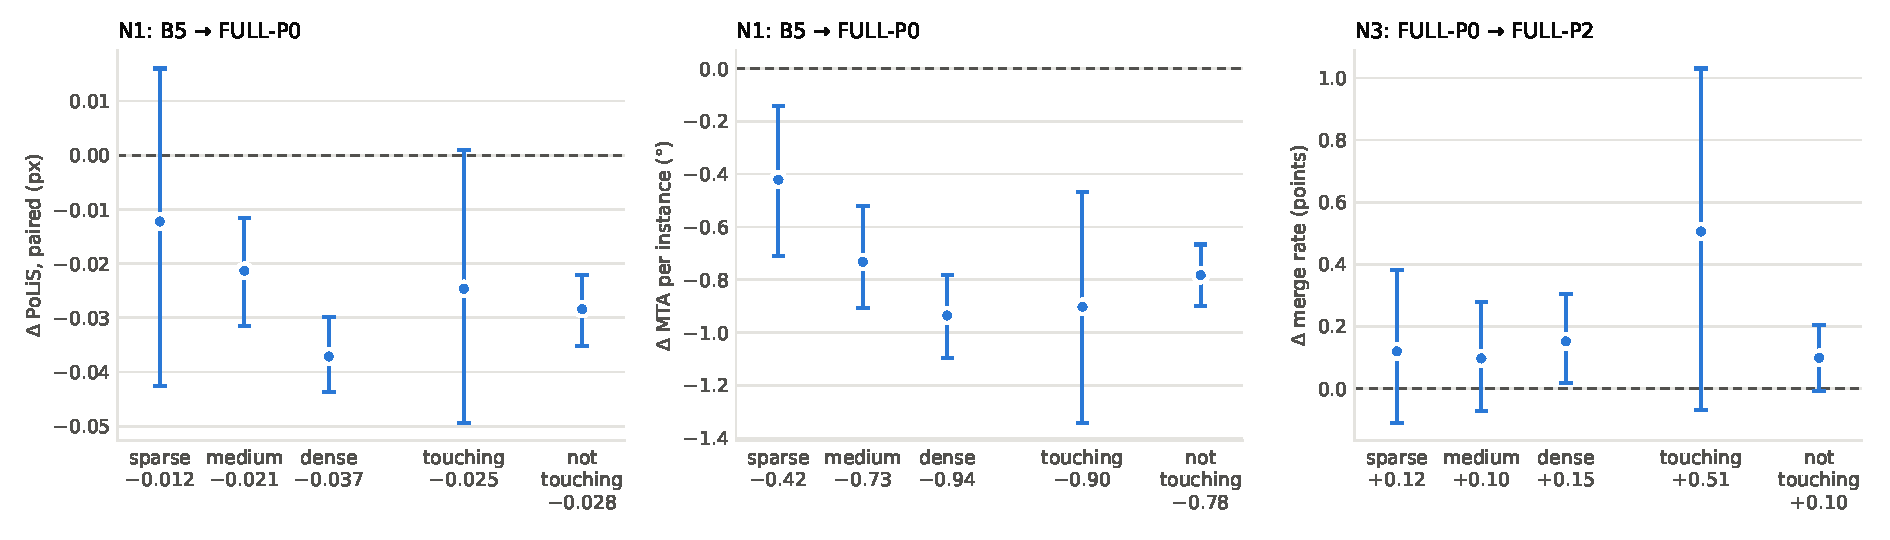
\includegraphics[width=0.95\textwidth]{figures/crowdai_n2}
\caption{The effects of Table~\ref{tab:density} per stratum, with 95\% bootstrap intervals.}
\label{fig:density}
\end{figure*}
The gain from the orientation head grows from sparse to dense tiles on both metrics (Table~\ref{tab:density},
Fig.~\ref{fig:density}). The difference between the dense and the sparse effect is significant for the MTA,
$\NDenseMta^\circ$, $\NDenseMtaCi$, but not for the PoLiS, $\NDensePolis$\,px, $\NDensePolisCi$. Our rule asks for both,
so ``largest in dense areas'' is not supported as a claim; the trend is there for one metric and has the same sign for
the other.

\subsection{Contact class}
\label{sec:contact}
Contact pixels are about 0.01\% of the building pixels. In \NContactInactive{} of the \NContactRuns{} FULL runs the
contact class is never the most probable class on the selection split, and its probability stays near zero everywhere.
In those runs buildings are separated only by predicted background gaps. Whether the class is active does not predict
the merge rate across seeds. The orientation-head comparison is unaffected in the seed where the class is active in
both models, but the finding means that the mechanism we adopted for touching roofs is mostly not at work.

\subsection{Comparison on leakage-free data}
\begin{table*}[t]
\centering
\caption{HiSup, evaluated from its released predictions, and our final model on the \NTilesClean{} validation tiles
without a duplicate in the training set. Same evaluation code for both.}
\label{tab:sota}
\resizebox{\textwidth}{!}{% sota: from tables/crowdai/sota.json (git 521cba53c565, 2026-11-12T14:39:44+07:00); do not edit
\begin{tabular}{l c cccccccc}
\toprule
Method & Polygon labels & AP & AP$_{50}$ & AP$_b$ & IoU & PoLiS$\downarrow$ & MTA$\downarrow$ & C-IoU & N-ratio \\
\midrule
HiSup (released predictions) & yes & 65.60 & 87.29 & 43.97 & 89.92 & 1.364 & 34.54 & 81.25 & 1.06 \\
FULL-P0 (ours) & no & 61.14\,{\scriptsize$\pm$0.98} & 86.15\,{\scriptsize$\pm$0.10} & 35.19\,{\scriptsize$\pm$1.79} & 87.54\,{\scriptsize$\pm$0.37} & 1.825\,{\scriptsize$\pm$0.073} & 36.18\,{\scriptsize$\pm$0.48} & 73.29\,{\scriptsize$\pm$0.63} & 1.29\,{\scriptsize$\pm$0.04} \\
\midrule
$\Delta$ (ours $-$ HiSup) &  & $-4.45$ {\scriptsize$[-5.73,\,-3.44]$} &  & $-8.79$ {\scriptsize$[-10.55,\,-7.41]$} & $-2.37$ {\scriptsize$[-2.74,\,-1.95]$} & $+0.461$ {\scriptsize$[+0.325,\,+0.587]$} & $+1.65$ {\scriptsize$[+0.97,\,+2.30]$} & $-7.95$ {\scriptsize$[-9.32,\,-6.55]$} &  \\
\bottomrule
\end{tabular}
}
\end{table*}
\begin{table}[t]
\centering
\caption{Numbers \emph{reported in the cited papers} on the full CrowdAI validation set, which leaks from the training
set. They are not comparable with Tables~\ref{tab:ablation} and~\ref{tab:sota}.}
\label{tab:reported}
\resizebox{\columnwidth}{!}{% reported: from tables/crowdai/paper.json (git 521cba53c565, 2026-11-12T14:39:44+07:00); do not edit
\begin{tabular}{l ccccccccc}
\toprule
Method (as reported) & AP & AP$_{50}$ & AP$_{75}$ & AR & AP$_b$ & IoU & C-IoU & PoLiS$\downarrow$ & MTA$\downarrow$ \\
\midrule
HiSup, HRNetV2-W48 & 79.4 & 92.7 & 85.3 & 81.5 & 66.5 & 94.3 & 89.6 & 0.726 & -- \\
FFL, UResNet101 (with field), frame field polygonization & 61.3 & 87.5 & 70.6 & 65.0 & -- & -- & -- & -- & 31.9 \\
PolyWorld (offset on), R2U-Net & 63.3 & 88.6 & 70.5 & 75.4 & -- & 91.3 & 88.2 & -- & 32.9 \\
PolyR-CNN, Swin-Base & 79.2 & 97.4 & 90 & 85.2 & 63.3 & 91.6 & -- & 1.204 & -- \\
Pix2Poly & 79.6 & 91.6 & 85.2 & 87.7 & -- & 95.03 & 89.85 & 0.479 & 23.1 \\
\bottomrule
\end{tabular}
}
\end{table}
Our evaluation reproduces the reported AP of HiSup on the full validation set, \NLeakyApHisup{}
(Table~\ref{tab:reported} lists the reported numbers). On the clean tiles the same predictions score \NCleanApHisup{}
(Table~\ref{tab:sota}). The clean tiles are not a random sample of the validation set, so part of the drop may come from
their difficulty and not only from leakage; still, the reported level does not carry over. FULL-P0, trained without
polygon annotations and on the deduplicated training split, is $\NCleanDeltaAp$ AP behind, $\NCleanDeltaApCi$, more than
the 3 points we had set as the limit: ``close to the state of the art'' is not supported. The two are close in
AP$_{50}$ (\NCleanApfiftyFull{} against \NCleanApfiftyHisup) and apart in boundary accuracy: our pipeline finds the same
buildings and places their outlines less precisely.

\subsection{WHU}
\begin{table}[t]
\centering
\caption{WHU test patches under the rules of Pix2Poly. $^\dagger$Reported in~\cite{adimoolam2025pix2poly}; their test
tiles are not exactly ours, so the comparison is approximate.}
\label{tab:whu}
\resizebox{\columnwidth}{!}{% whu: from tables/whu/p2p.json (git 521cba53c565, 2026-11-12T14:44:24+07:00); do not edit
\begin{tabular}{l l ccccc}
\toprule
Method & Ground truth & IoU & C-IoU & N-ratio & PoLiS$\downarrow$ & MTA$\downarrow$ \\
\midrule
FULL-P0 (ours) & Pix2Poly-style & 83.92 & 66.83 & 1.72 & 1.575 & 39.74 \\
FULL-P0 (ours) & official buildings & 84.22 & 67.01 & 1.72 & 1.496 & 39.10 \\
\midrule
Pix2Poly$^\dagger$ & Pix2Poly-style & 89.15 & 81.63 & 1.15 & 1.082 & 31.64 \\
HiSup (as evaluated in the Pix2Poly paper)$^\dagger$ & Pix2Poly-style & 87.12 & 79.62 & 1.15 & 1.158 & 34.75 \\
FFL, $\epsilon=$1.0 (as evaluated in the Pix2Poly paper)$^\dagger$ & Pix2Poly-style & 77.64 & 54.52 & 2.31 & 1.747 & 35.79 \\
FFL, $\epsilon=$0.125 (as evaluated in the Pix2Poly paper)$^\dagger$ & Pix2Poly-style & 77.61 & 32.19 & 5.09 & 1.783 & 35.27 \\
\bottomrule
\end{tabular}
}
\end{table}
On WHU (one seed) FULL-P0 reaches \NWhuAp{} AP and \NWhuCiouMain{} C-IoU against the official per-building ground
truth. Under the rules of Pix2Poly its C-IoU is \NWhuCiou, between the reported values of frame field learning and of
HiSup (\NWhuCiouHisup) and Pix2Poly (\NWhuCiouPixtopoly), see Table~\ref{tab:whu}. The effect of guiding the
regularization with the head has the same sign and the same growth with density as on CrowdAI. Touching buildings remain
the weak point: \NWhuMergeTouching\% of them are merged in patches with touching buildings.

\subsection{Exploratory: a binary baseline and detector seeds}
\label{sec:exploratory}
\begin{table*}[t]
\centering
\caption{Comparisons added after the results (exploratory, except FULL-P0 $\rightarrow$ FULL+Y, which was planned): paired
differences on all test tiles with 95\% bootstrap intervals. B3m: mode \emph{mar} on the components of B3; +Y: detector
seeds.}
\label{tab:exploratory}
\resizebox{\textwidth}{!}{% exploratory: from tables/crowdai/exploratory.json (git f96e54a20f99, 2026-11-12T20:27:37+07:00); do not edit
\begin{tabular}{l cccccc}
\toprule
Step & $\Delta$AP & $\Delta$C-IoU & $\Delta$Merge & $\Delta$Split & $\Delta$PoLiS & $\Delta$MTA \\
\midrule
B3 $\rightarrow$ B3m & $-0.85$ {\scriptsize$[-1.01,\,-0.70]$} & $+10.46$ {\scriptsize$[+10.09,\,+10.81]$} & $-0.03$ {\scriptsize$[-0.06,\,-0.00]$} & $+0.01$ {\scriptsize$[-0.01,\,+0.02]$} & $-0.042$ {\scriptsize$[-0.046,\,-0.038]$} & $-9.39$ {\scriptsize$[-9.55,\,-9.23]$} \\
B3m $\rightarrow$ FULL-P0 & $-2.95$ {\scriptsize$[-3.15,\,-2.65]$} & $-2.42$ {\scriptsize$[-2.67,\,-2.16]$} & $-0.85$ {\scriptsize$[-1.01,\,-0.67]$} & $+1.52$ {\scriptsize$[+1.37,\,+1.66]$} & $+0.138$ {\scriptsize$[+0.130,\,+0.147]$} & $+0.39$ {\scriptsize$[+0.26,\,+0.51]$} \\
FULL-P0 $\rightarrow$ FULL+Y & $-0.07$ {\scriptsize$[-0.24,\,+0.05]$} & $-0.07$ {\scriptsize$[-0.12,\,-0.04]$} & $-0.45$ {\scriptsize$[-0.56,\,-0.35]$} & $+0.24$ {\scriptsize$[+0.19,\,+0.30]$} & $+0.008$ {\scriptsize$[+0.003,\,+0.014]$} & $-0.01$ {\scriptsize$[-0.02,\,-0.00]$} \\
B3m $\rightarrow$ B3m+Y & $-0.10$ {\scriptsize$[-0.28,\,+0.20]$} & $-0.08$ {\scriptsize$[-0.13,\,-0.04]$} & $-0.67$ {\scriptsize$[-0.82,\,-0.53]$} & $+0.36$ {\scriptsize$[+0.30,\,+0.44]$} & $+0.003$ {\scriptsize$[-0.002,\,+0.008]$} & $-0.01$ {\scriptsize$[-0.01,\,-0.00]$} \\
B3m+Y $\rightarrow$ FULL+Y & $-2.92$ {\scriptsize$[-3.17,\,-2.72]$} & $-2.41$ {\scriptsize$[-2.65,\,-2.15]$} & $-0.63$ {\scriptsize$[-0.76,\,-0.49]$} & $+1.39$ {\scriptsize$[+1.25,\,+1.54]$} & $+0.144$ {\scriptsize$[+0.136,\,+0.154]$} & $+0.38$ {\scriptsize$[+0.26,\,+0.50]$} \\
\bottomrule
\end{tabular}
}
\end{table*}
Because B3 has the highest AP, we applied the regularization of mode \emph{mar} directly to its connected components
(B3m). This costs $\NRegBinaryAp$ AP and raises the C-IoU by $\NRegBinaryCiou$ points (Table~\ref{tab:exploratory}).
B3m is better than FULL-P0 on every metric except merged buildings: FULL-P0 is $\NBinaryToFullAp$ AP and
$\NBinaryToFullCiou$ C-IoU behind it, and splits more buildings, while its merge rate is lower (\NMergeFull\% against
\NMergeBthreem\%; in tiles with touching buildings \NMergeTouchingFull\% against \NMergeTouchingBthreem\%). The
three-class route buys separation at the price of boundary accuracy.

Detector seeds address the remaining weakness of both. The detector reaches a mAP$_{50}$ of \NDetectorMap{} on the
selection split. Its seeds lower the merge rate of FULL-P0 by $\NSeedFullMerge$ points, $\NSeedFullMergeCi$, and of B3m
by $\NSeedBinaryMerge$ points, $\NSeedBinaryMergeCi$, in every seed, and more in tiles with touching buildings. They
also split more buildings, and AP does not change. The ranking of the two routes stays the same.

Fig.~\ref{fig:qualitative} shows the polygons of four models on test tiles.

\begin{figure*}[t]
\centering
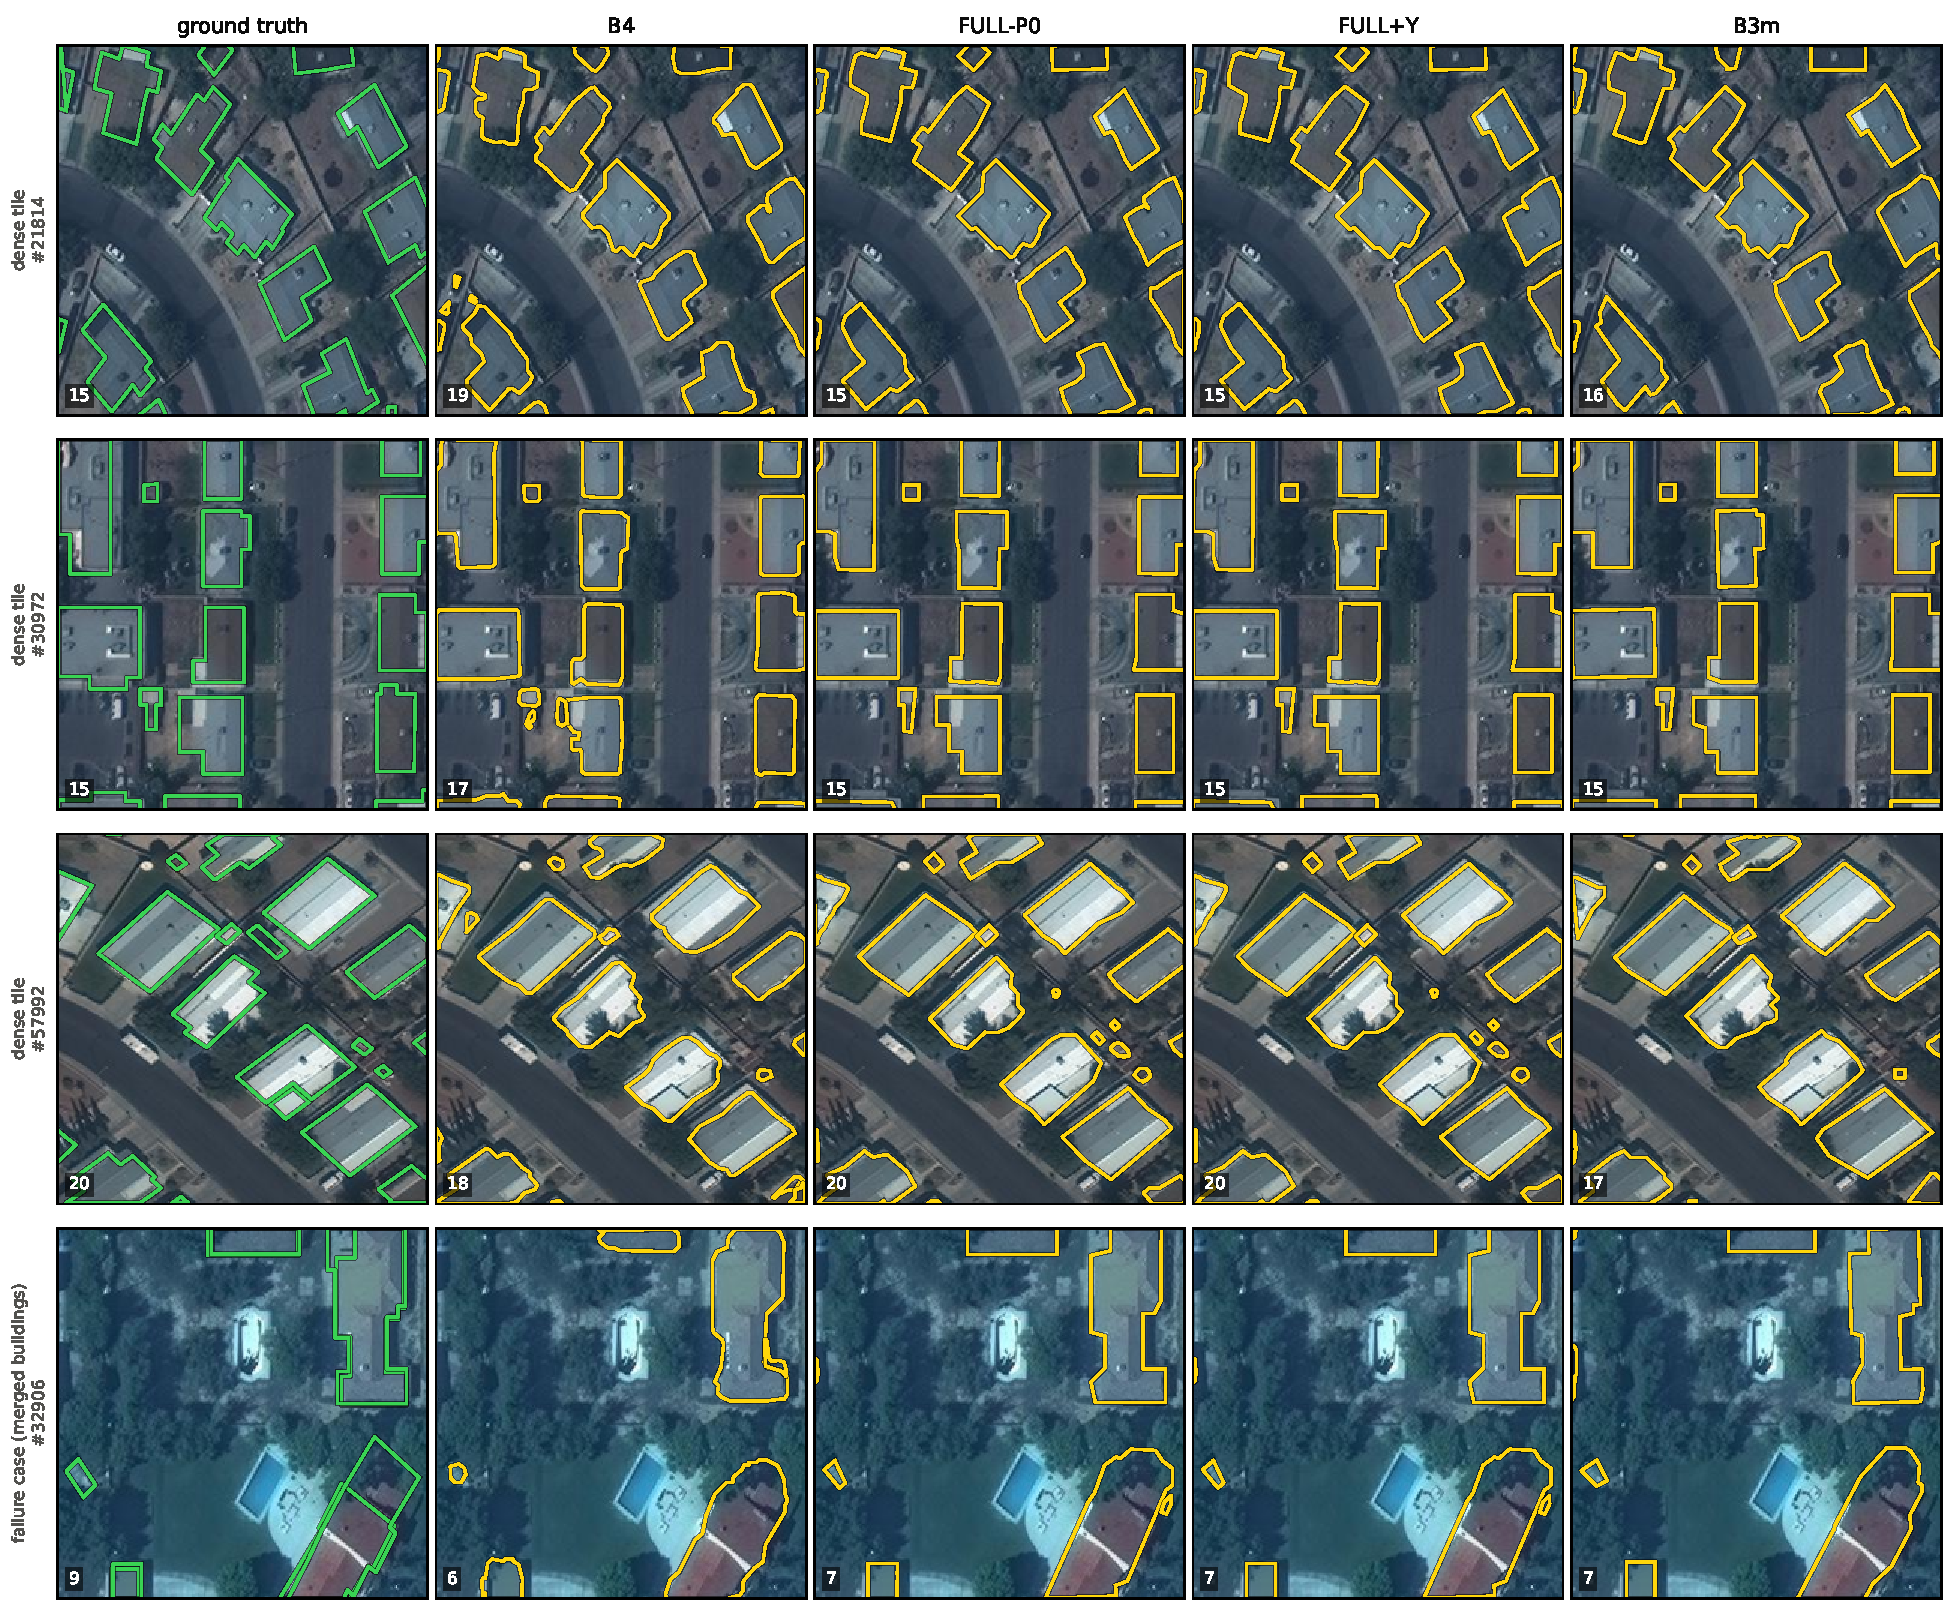
\includegraphics[width=0.92\textwidth]{figures/crowdai_qualitative}
\caption{Test tiles of the dense stratum (three rows, drawn at random) and, in the last row, the tile with touching
buildings on which FULL-P0 merges the most buildings. The number in each panel counts its polygons. B4 draws raw
contours; the other models regularize them.}
\label{fig:qualitative}
\end{figure*}

\subsection{Cost}
\begin{table}[t]
\centering
\caption{Cost on an RTX 5090 and one CPU thread for the post-processing. The detector's parameters are not included.}
\label{tab:efficiency}
\resizebox{\columnwidth}{!}{% efficiency: from tables/crowdai/efficiency.json (git f96e54a20f99, 2026-11-12T20:27:37+07:00); do not edit
\begin{tabular}{l ccccc}
\toprule
Code & Params (M) & Network FPS & Post-proc. (ms) & Detector (ms) & Pipeline FPS \\
\midrule
B3 & 20.81 & 124.6 & 5.48 & -- & 74.0 \\
B4 & 20.81 & 125.1 & 8.59 & -- & 60.3 \\
FULL-P0 & 20.81 & 128.9 & 15.89 & -- & 42.3 \\
FULL-P2 & 20.81 & 128.7 & 16.11 & -- & 41.9 \\
FULL+Y & 20.81 & 124.0 & 17.17 & 2.23 & 36.4 \\
\bottomrule
\end{tabular}
}
\end{table}
All networks have about \NParamsFull{} million parameters (Table~\ref{tab:efficiency}). The orientation-guided
regularization dominates the post-processing time; the whole pipeline runs at \NFpsFull{} tiles per second, and at
\NFpsFullY{} with the detector.

\section{Discussion and Limitations}
The orientation head does what it was designed for, but the effect is small, and the larger share of the polygon
quality comes from the regularization itself, which works as well with rectangles fitted to the predicted instances.
The head was only tested on the three-class route; whether it helps the stronger binary route needs a training run we
did not plan.

The clean comparison rests on \NTilesClean{} tiles that are not a random sample. WHU has one seed and an approximate
match to the published test set. The detector was trained once and shared by the three seeds, and its confidence
threshold was chosen at the upper end of a grid fixed in advance. Polygons have no holes. The deduplication relies on
perceptual hashes and can miss near-duplicates that differ by more than a rotation or flip.

\section{Conclusion}
With instance masks only, a segmentation network and a geometric regularization give polygons whose complexity is close
to the ground truth, $\NCleanDeltaAp$ AP from a polygon-supervised method on leakage-free data. An orientation head
supervised by rectangles fitted to the masks improves the geometry a little, and more in dense tiles. Morphological
priors and a contact class do not deliver the separation of touching roofs they were meant to; seeds from a
mask-supervised detector do. The strongest pipeline we found is also the simplest, a binary segmentation with
regularized components, which we could only identify because the baselines were evaluated under the same protocol as
the method.

\bibliographystyle{IEEEtran}
\bibliography{refs}

\end{document}
